\p
تعداد مثلث‌ها در مثلث‌بندی برابر
$n - 2$
است (‌زیرا با رسم هر قطر یکی به تعداد نواحی افزوده می‌شود و لذا پس از رسم
$n - 3$
قطر تعداد نواحی برابر
$n - 2$
می‌شود). حال
$n$ 
ضلع
$n$
ضلعی در
$n - 2$
مثلث قرار دارند و چون هر مثلث حداقل یکی از اضلاع
$n$
ضلعی را دارد، لذا دقیقا دو تا از مثلث‌ها دو ضلع از
$n$
ضلعی  بقیه هر کدام یک ضلع از
$n$
ضلعی را دارند(البته توجه کنید هیچ مثلثی سه ضلع از
$n$
ضلعی را ندارد).
\begin{center}
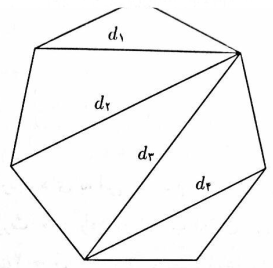
\includegraphics[height=6.5cm]{1.png}
\end{center}
لذا برای ساختن یک مثلث‌بندی با ویژگی‌ مورد نظر ابتدا یک راس مانند
$A$
از
$n$
ضلعی را انتخاب و دو راس مجاور با آن را با قطر
$d_1$
به هم وصل می‌کنیم. این کار به
$n$
طریق قابل انجام است. حال مثلث شامل
$d_1$
از سمت دیگر باید یک ضلع از
$n$
ضلعی را داشته باشد، لذا ضلع سوم این مثلث باید یکی از دو قطری باشد که یک انتهای
$d_1$
را به راس مجاور با انتهای دیگر وصل می‌کند. لذا
$2$
انتخاب برای رسم قطر 
$d_2$
وجود دارد. با استدلال مشابه نتیجه می‌گیریم برای رسم هر یک از قطرهای
$d_3, \cdots, d_{n-3}$
نیز
$2$
انتخاب وجود دارد. لذا
$n2^{n-4}$
روش برای انتخاب راس
$A$
و رسم قطرهای
$d_1, 2, \cdots, d_{n-3}$
وجود دارد. حال توجه کنید که هر مثلث‌بندی با ویژگی‌های مورد نظر دوبار در این روش شمرده می‌شود، لذا پاسخ مسئله برابر
$n2^{n-5}$
است.